% Auto-generated by experiments.analysis.generate_win_counts --slides --- do not edit.
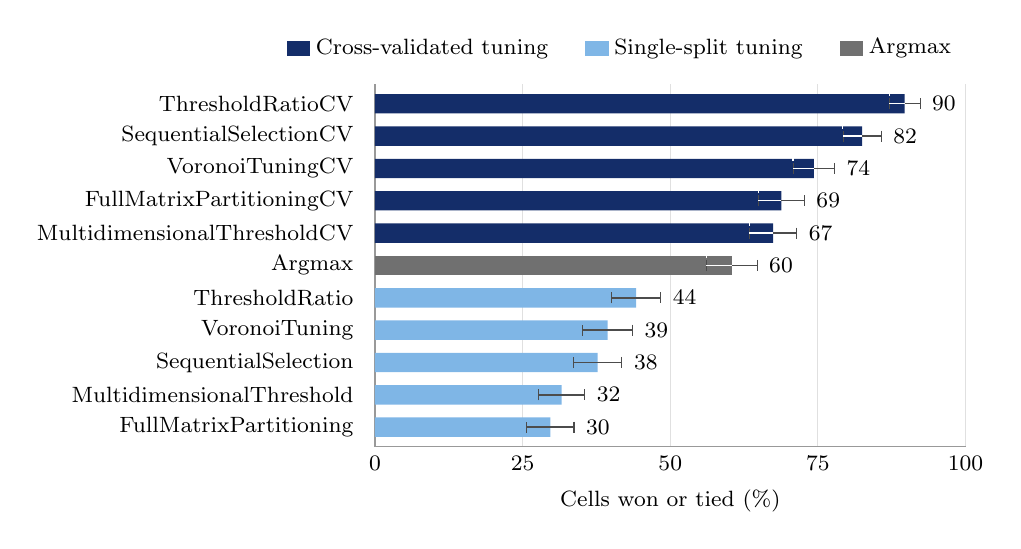
\begin{tikzpicture}
\definecolor{winbarcv}{HTML}{142D69}
\definecolor{winbarsplit}{HTML}{7FB6E6}
\definecolor{winbaranalytical}{HTML}{E6AF3C}
\definecolor{winbarargmax}{HTML}{707070}
\begin{axis}[
    xbar, bar shift=0pt, bar width=7pt,
    scale only axis, width=7.5cm, height=4.60cm,
    xmin=0, xmax=100, xtick={0,25,50,75,100},
    xlabel={Cells won or tied (\%)},
    ymin=0.4, ymax=11.6, y dir=reverse,
    ytick={1,2,3,4,5,6,7,8,9,10,11},
    yticklabels={ThresholdRatioCV,SequentialSelectionCV,VoronoiTuningCV,FullMatrixPartitioningCV,MultidimensionalThresholdCV,Argmax,ThresholdRatio,VoronoiTuning,SequentialSelection,MultidimensionalThreshold,FullMatrixPartitioning},
    axis x line*=bottom, axis y line*=left,
    axis line style={draw=black!40},
    tick style={draw=none},
    xmajorgrids=true,
    major grid style={draw=black!12, line width=0.3pt},
    tick label style={font=\footnotesize},
    label style={font=\footnotesize},
    clip=false,
    legend columns=3,
    legend cell align=left,
    legend image code/.code={\fill[#1] (0cm,-0.1cm) rectangle (0.3cm,0.1cm);},
    legend style={draw=none, fill=none, font=\footnotesize,
        at={(1,1.04)}, anchor=south east,
        /tikz/every even column/.append style={column sep=0.4cm}},
]
\addplot[fill=winbarcv, draw=none, error bars/x dir=both, error bars/x explicit, error bars/error bar style={black!70, line width=0.5pt}] coordinates { (89.7,1) +- (2.6,0) (82.5,2) +- (3.2,0) (74.3,3) +- (3.5,0) (68.8,4) +- (3.9,0) (67.4,5) +- (4.0,0) };
\addlegendentry{Cross-validated tuning}
\addplot[fill=winbarsplit, draw=none, error bars/x dir=both, error bars/x explicit, error bars/error bar style={black!70, line width=0.5pt}] coordinates { (44.2,7) +- (4.2,0) (39.4,8) +- (4.2,0) (37.7,9) +- (4.1,0) (31.6,10) +- (3.9,0) (29.7,11) +- (4.0,0) };
\addlegendentry{Single-split tuning}
\addplot[fill=winbarargmax, draw=none, error bars/x dir=both, error bars/x explicit, error bars/error bar style={black!70, line width=0.5pt}] coordinates { (60.4,6) +- (4.3,0) };
\addlegendentry{Argmax}
\draw[white, line width=0.5pt] (axis cs:89.7,1) -- (axis cs:87.1,1) +(0,-2pt) -- +(0,2pt);
\draw[white, line width=0.5pt] (axis cs:82.5,2) -- (axis cs:79.2,2) +(0,-2pt) -- +(0,2pt);
\draw[white, line width=0.5pt] (axis cs:74.3,3) -- (axis cs:70.8,3) +(0,-2pt) -- +(0,2pt);
\draw[white, line width=0.5pt] (axis cs:68.8,4) -- (axis cs:64.9,4) +(0,-2pt) -- +(0,2pt);
\draw[white, line width=0.5pt] (axis cs:67.4,5) -- (axis cs:63.4,5) +(0,-2pt) -- +(0,2pt);
\draw[white, line width=0.5pt] (axis cs:60.4,6) -- (axis cs:56.1,6) +(0,-2pt) -- +(0,2pt);
\node[anchor=west, font=\footnotesize, inner sep=1pt] at (axis cs:93.8,1) {90};
\node[anchor=west, font=\footnotesize, inner sep=1pt] at (axis cs:87.2,2) {82};
\node[anchor=west, font=\footnotesize, inner sep=1pt] at (axis cs:79.3,3) {74};
\node[anchor=west, font=\footnotesize, inner sep=1pt] at (axis cs:74.2,4) {69};
\node[anchor=west, font=\footnotesize, inner sep=1pt] at (axis cs:72.9,5) {67};
\node[anchor=west, font=\footnotesize, inner sep=1pt] at (axis cs:66.2,6) {60};
\node[anchor=west, font=\footnotesize, inner sep=1pt] at (axis cs:49.9,7) {44};
\node[anchor=west, font=\footnotesize, inner sep=1pt] at (axis cs:45.1,8) {39};
\node[anchor=west, font=\footnotesize, inner sep=1pt] at (axis cs:43.3,9) {38};
\node[anchor=west, font=\footnotesize, inner sep=1pt] at (axis cs:37.0,10) {32};
\node[anchor=west, font=\footnotesize, inner sep=1pt] at (axis cs:35.2,11) {30};
\end{axis}
\end{tikzpicture}%
